\documentclass[11pt]{article}
\usepackage[letterpaper,margin=0.85in]{geometry}
\usepackage[T1]{fontenc}
\usepackage{lmodern}
\usepackage{amsmath,amssymb,graphicx,booktabs,array,tabularx}
\usepackage[hidelinks]{hyperref}
\usepackage{microtype}
\setlength{\parindent}{0pt}
\setlength{\parskip}{4pt}
\setlength{\textfloatsep}{10pt}\setlength{\intextsep}{10pt}
\makeatletter\renewcommand\section{\@startsection{section}{1}{0pt}{-2ex plus -.5ex minus -.2ex}{1ex plus .2ex}{\normalfont\Large\bfseries}}\makeatother
\setlength{\emergencystretch}{2em}
\renewcommand{\topfraction}{0.9}\renewcommand{\textfraction}{0.08}
\hypersetup{pdftitle={Early insulin delivery and fixed-dose design trade-offs in a proposed human-scale islet implant},pdfauthor={UCP Technology LLC}}
\begin{document}
\begin{center}{\LARGE\bfseries Early insulin delivery and fixed-dose design trade-offs in a proposed human-scale islet implant}\\[10pt]UCP Technology LLC\\26 October 2026\end{center}
\section*{Abstract}
Insulin production and delivery across an implant boundary are distinct engineering endpoints. We calculate the transfer response of the proposed seven-pouch BEAM human-scale geometry and its fixed-dose design requirements. Uniform production maintained for 30 minutes in 0.75 mm annuli gives 71.53\% delivery with assumed diffusivity 3.0 \ensuremath{\times} 10\textsuperscript{-}\textsuperscript{1}\textsuperscript{0} m\textsuperscript{2}/s and perfect outer/end sinks. Continuum and finite-volume calculations agree to about 0.0012 percentage points. A nominal 0.60 mm redesign reaches 80.21\% but falls below 80\% with reflecting ends or a 5\% diffusivity reduction. Reoptimized 80\% choices require 141.18 cm\textsuperscript{2} lateral area under favorable assumptions, 240.09 cm\textsuperscript{2} with lower diffusivity alone, 289.12 cm\textsuperscript{2} with finite outer permeability alone, and 381.79 cm\textsuperscript{2} with both changes and reflecting ends. A declared 24-scenario set selects the same 0.21 mm design. If a hypothetical minimum thickness of 0.25 or 0.30 mm is imposed, the highest worst-scenario delivery on the remaining grid is only 75.90\% or 69.67\%; the 80\% target becomes unattainable within that constrained family. These assumed constraints do not identify a biological thickness limit. The device-specific map distinguishes additional area requirements from loss of target attainability and identifies the transport and packing measurements needed to choose among scenarios.

\section*{1 Introduction}
Islet encapsulation must preserve viable insulin-secreting cells while permitting timely transport. Pham and colleagues reported the continuously oxygenated macroencapsulation platform BEAM and proposed a seven-pouch human-scale configuration [1]. The proposal supplies dimensions and a dose target, but its human-scale drawing is not a human efficacy experiment. Its hour-long static secretion assays also do not directly determine how a new production increment crosses the proposed geometry during the first 30 minutes.

Secretion--transport coupling, geometry-dependent delay and pressure-driven improvement are established [2--5]. For the later BEAM proposal, the present map connects a reconciled dose and geometry to actual finite annular segments, timed boundary delivery and the costs of redesign. It lets a reader determine which assumed transport conditions require more area and whether a specified minimum layer thickness removes every target-meeting design from the sampled family. Table 1 distinguishes this device-specific decision from the earlier general transport and geometry results.

\par\begin{table}[htbp]\centering\small Table 1. Closest prior work and the specific added output here.\\[4pt]\begin{tabularx}{\linewidth}{>{\raggedright\arraybackslash}X>{\raggedright\arraybackslash}X>{\raggedright\arraybackslash}X>{\raggedright\arraybackslash}X>{\raggedright\arraybackslash}X}\toprule
Study / geometry & Source input & Endpoint & Experimental basis / validation & Additional output here\\\midrule
Buchwald [2]; encapsulated islets & Glucose-driven secretion & Dynamic insulin release & Dynamic release experiments and coupled model & Later BEAM proposal; explicit fixed-dose segments\\
Ernst [3]; SHARP device designs & Islet size/position and oxygen-consumption inputs & Oxygen-limited functional capacity & Computational platform with experimental comparisons & Uniform-source timing isolated from oxygen function\\
Thomson [4]; macroencapsulation chambers & Stimulus-linked production / transport & Insulin delivery dynamics & Pressure-driven transport and device experiments & Passive finite-annulus map at stated BEAM dose\\
Trask [5]; reservoir, membrane and tissue & Initial insulin bolus & External transport; fibrosis and flow & Measured tracer membrane inputs; no direct experimental device-response validation & Continuous-input convolution and fixed-dose BEAM design map\\
\bottomrule\end{tabularx}\end{table}\par
\section*{2 Geometry, parameters and measurement boundaries}
An islet equivalent (IEQ) is the conventional volume of a 150 \ensuremath{\mu}m diameter spherical islet; it is not a count of physically identical spheres. Let a and b be inner and outer annular radii, h = b \ensuremath{-} a the layer thickness, L the active segment length, N the total IEQ dose, \ensuremath{\rho} the effective IEQ loading density, and s\textsubscript{0} the uniform incremental production per volume and time. Nominally there are seven segments with a = 3.00 mm, b = 3.75 mm, h = 0.75 mm and L = 70 mm. Straight annular ends and homogeneous loading idealize the rounded proposal; they do not reconstruct device CAD or actual cell positions (Figure 1).

\par\begin{table}[htbp]\centering\small Table 2. Parameter and assumption provenance.\\[4pt]\begin{tabularx}{\linewidth}{>{\raggedright\arraybackslash}X>{\raggedright\arraybackslash}X>{\raggedright\arraybackslash}X>{\raggedright\arraybackslash}X}\toprule
Quantity & Value used & Provenance class & Qualification\\\midrule
Outer diameter; layer; length; count & 7.5 mm; 0.75 mm; 70 mm; 7 & Reported proposal [1] & Supplementary Fig.24, p.21; not measured as-built geometry\\
Dose N & 420,000 IEQ & Reported target [1] & Held fixed in every redesign\\
Active volume; effective \ensuremath{\rho} & 7.7931 mL; 53,893.7 IEQ/mL & Derived & Straight annuli; dose/volume\\
Nominal D & 3.0 \ensuremath{\times} 10\textsuperscript{-}\textsuperscript{1}\textsuperscript{0} m\textsuperscript{2}/s & Assumed scenario & No measured BEAM-gel value; not a universal maximum\\
D sensitivity & 1.0, 2.0, 2.85, 3.0 \ensuremath{\times} 10\textsuperscript{-}\textsuperscript{1}\textsuperscript{0} m\textsuperscript{2}/s & Assumed scenarios & Selected sensitivity points; no distribution or empirical coverage\\
Outer permeability P & 10\textsuperscript{-}\textsuperscript{6}, 10\textsuperscript{-}\textsuperscript{5} m/s; perfect sink & Assumed scenarios & No fitted assembled-device values\\
Ends; source; receiving medium & Absorbing/reflecting; uniform; zero background increment & Structural assumptions & No tissue transport, heterogeneous secretion or feedback\\
Transport calibration in this geometry & None & Not measured & Literature measurements belong to other systems\\
\bottomrule\end{tabularx}\end{table}\par
The straight-annulus volume at the separate reported 60,000 IEQ/mL would imply 467,586.8 IEQ. Even the rounded caption arithmetic, 7 \ensuremath{\times} 1.11 mL \ensuremath{\times} 60,000 IEQ/mL, gives 466,200 IEQ rather than 420,000 IEQ. We preserve the stated dose by recalculating effective density. Unfilled volume, rounded ends or other details could matter, but no explanation is assigned without evidence. This discrepancy rescales capacity and oxygen accounting; it does not change a normalized linear delivery fraction with a fixed spatial source.

\begin{figure}[htbp]\centering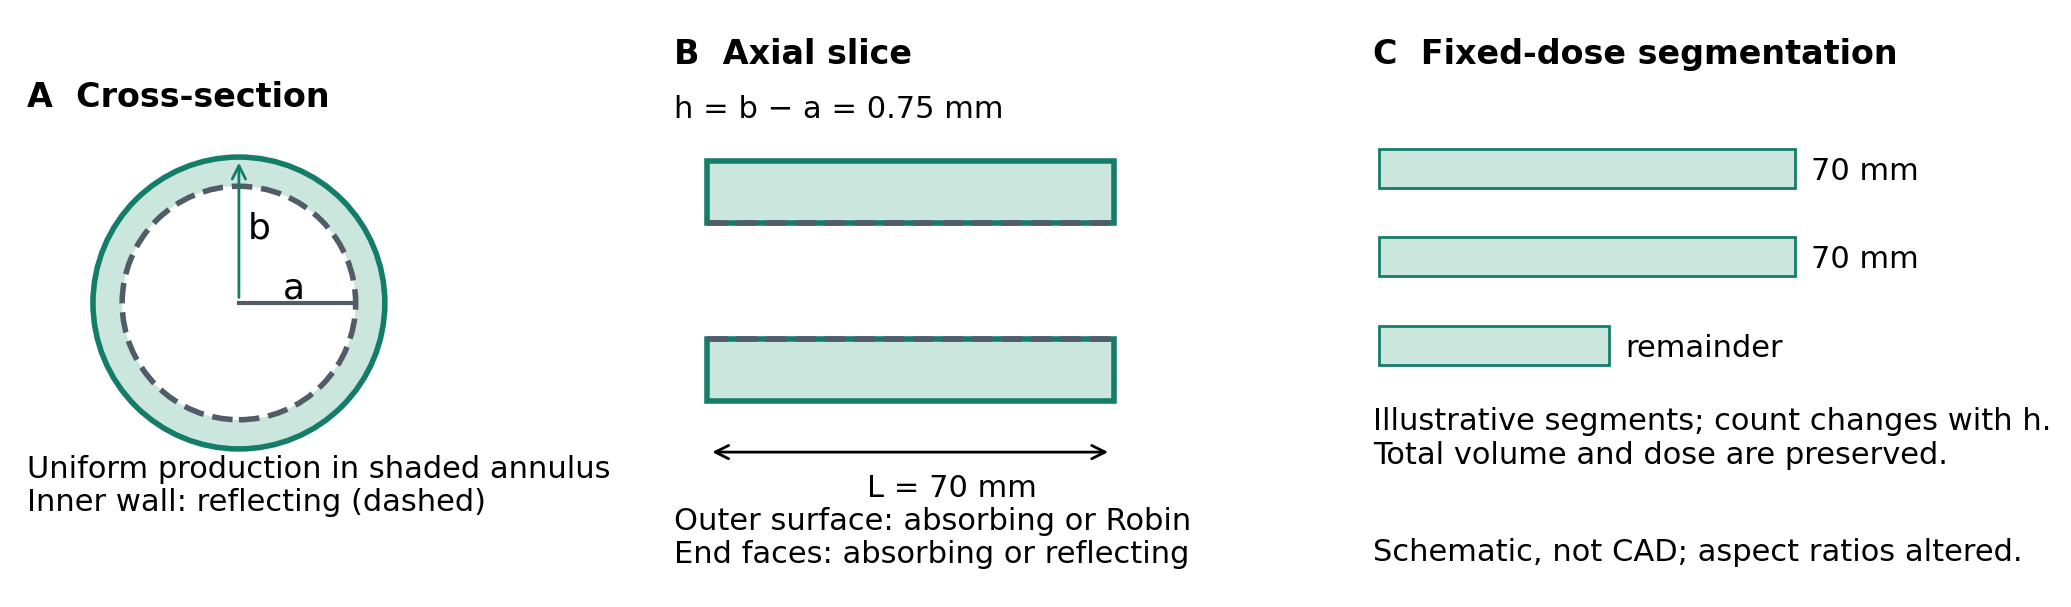
\includegraphics[width=0.9264705882352942\linewidth]{assets/geometry_schematic.png}\caption{Original model schematic. A: the shaded annulus produces insulin; the inner boundary reflects. B: the outer boundary is absorbing or Robin, and both ends are absorbing or reflecting. C: dose-preserving redesigns use full 70 mm segments and one remainder; the illustration does not specify a particular pouch count. The model excludes connectors and the oxygen generator.}\end{figure}
\section*{3 Transfer response and numerical methods}
For one segment, \ensuremath{\Omega} is a \ensuremath{\leq} r \ensuremath{\leq} b, 0 \ensuremath{\leq} z \ensuremath{\leq} L with rotational symmetry. Incremental concentration c is zero initially and obeys diffusion plus a spatially uniform source q(t)/V, where q is the total production rate and V the corresponding modeled volume. The inner wall has zero normal derivative. At the outer wall, the outward flux is \ensuremath{-}D\ensuremath{\partial}c/\ensuremath{\partial}n = Pc; a perfect sink is the limit c = 0. The end faces are either c = 0 or \ensuremath{\partial}c/\ensuremath{\partial}n = 0. Delivered mass counts the integrated outward flux on all accessible boundaries, not systemic insulin exposure.

\begin{equation}\partial_t c=D\left[r^{-1}\partial_r(r\partial_r c)+\partial_z^2c\right]+q(t)/V\end{equation}
\begin{equation}M_{\mathrm{out}}(T)=\int_0^T\!\int_{\partial\Omega}(-D\nabla c\cdot\mathbf{n})\,dA\,dt\end{equation}
Let S(t) be the remaining fraction after a uniformly distributed unit initial inventory evolves under the source-free transport operator. For zero initial incremental inventory, linearity gives the general cumulative response. A nonzero uniform initial amount M\textsubscript{0} would contribute M\textsubscript{0}[1 \ensuremath{-} S(T)] separately.

\begin{equation}M_{\mathrm{out}}(T)=\int_0^T q(u)\,[1-S(T-u)]\,du\end{equation}
Two observables are kept distinct. The continuous-source deadline fraction \ensuremath{\eta}(T) uses constant q = s\textsubscript{0}V until the chosen deadline T. The fixed-pulse recovery R\ensuremath{\tau}(t) uses q = s\textsubscript{0}V only for 0 < t \ensuremath{\leq} \ensuremath{\tau}, with \ensuremath{\tau} = 30 minutes, and normalizes by the fixed amount s\textsubscript{0}V\ensuremath{\tau}. Before pulse completion, R\ensuremath{\tau} counts recovery relative to that full eventual pulse; after shutoff its denominator stays unchanged. They coincide at T = t = \ensuremath{\tau}.

\begin{equation}\eta(T)=1-\frac{1}{T}\int_0^T S(v)\,dv,\qquad R_\tau(t)=\frac{M_{\mathrm{out}}(t)}{s_0V\tau}\end{equation}
The continuum implementation uses Bessel radial modes and odd sine axial modes for absorbing ends; reflecting ends retain only the zero axial mode. For a uniform source, the self-adjoint diffusion operator gives nonnegative modal weights. Radial Robin roots satisfy Dk f\textsubscript{1}(b) = Pf\textsubscript{0}(b), where f\textsubscript{0}(r) = J\textsubscript{0}(kr)Y\textsubscript{1}(ka) \ensuremath{-} Y\textsubscript{0}(kr)J\textsubscript{1}(ka) and f\textsubscript{1} = \ensuremath{-}f\textsubscript{0}\ensuremath{\prime}/k. Perfect outer sinks instead require f\textsubscript{0}(b) = 0. Survival is the sum of modal weights times their exponential decay. Actual segment responses are weighted by volume.

An independently constructed conservative finite-volume spatial operator uses cylindrical volumes and face conductances, including the outer resistance. Exact-time eigendecomposition avoids time-step error. Refinement, quadrature checks on continuum weights, positivity checks and independent face-flux integration test implementation and conservation. The primary continuum/FV difference is 0.00118 percentage points; the estimated primary numerical uncertainty is 0.00322 percentage points. Positive omitted-mode tails bound truncation, but numerical roots and floating-point guards do not form certified interval arithmetic. Full formulas and numerical values are in METHODS.md and the evidence files.

For the fixed perfect-sink geometry, changing D scales the diffusion clock; lower D cannot increase delivery. Adding passive resistance or reflecting a formerly absorbing face cannot advance first exit for the same source. These are conditional ordering statements. The simple clock-scaling proof does not apply unchanged at fixed finite P, because P/D changes. The Robin design map therefore evaluates every declared combination and claims robustness only across those discrete scenarios.

\section*{4 Delivery, waveform and the nominal design}
The nominal continuous-source calculation gives \ensuremath{\eta}(30 min) = 71.53\%, below the prespecified 80\% engineering benchmark. The benchmark has no demonstrated clinical acceptance meaning. At shutoff, 28.47\% remains in the implant; almost all of the fixed pulse has left by 150 minutes (Figure 2). For comparison, a uniform initial inventory gives 94.20\% recovery by 30 minutes. The two inputs can have equal total amount but have different molecule ages and peak-rate constraints; an ideal instantaneous bolus is not a demonstrated cellular secretion waveform.

The nominal diffusion scale h\textsuperscript{2}/D is 31.25 minutes and DT/h\textsuperscript{2} is 0.96 at 30 minutes. The deadline is therefore comparable with transport across the layer; this scale is not an identical exit time for every molecule. Moving production into the outer half or quarter of the same domain raises the modeled fraction to 82.05\% or 90.07\%, with local density multipliers 1.895 or 3.692. These source-placement cases explicitly rule out a placement-independent 72\% ceiling. They do not establish feasible cell packing or local oxygen supply.

\begin{figure}[htbp]\centering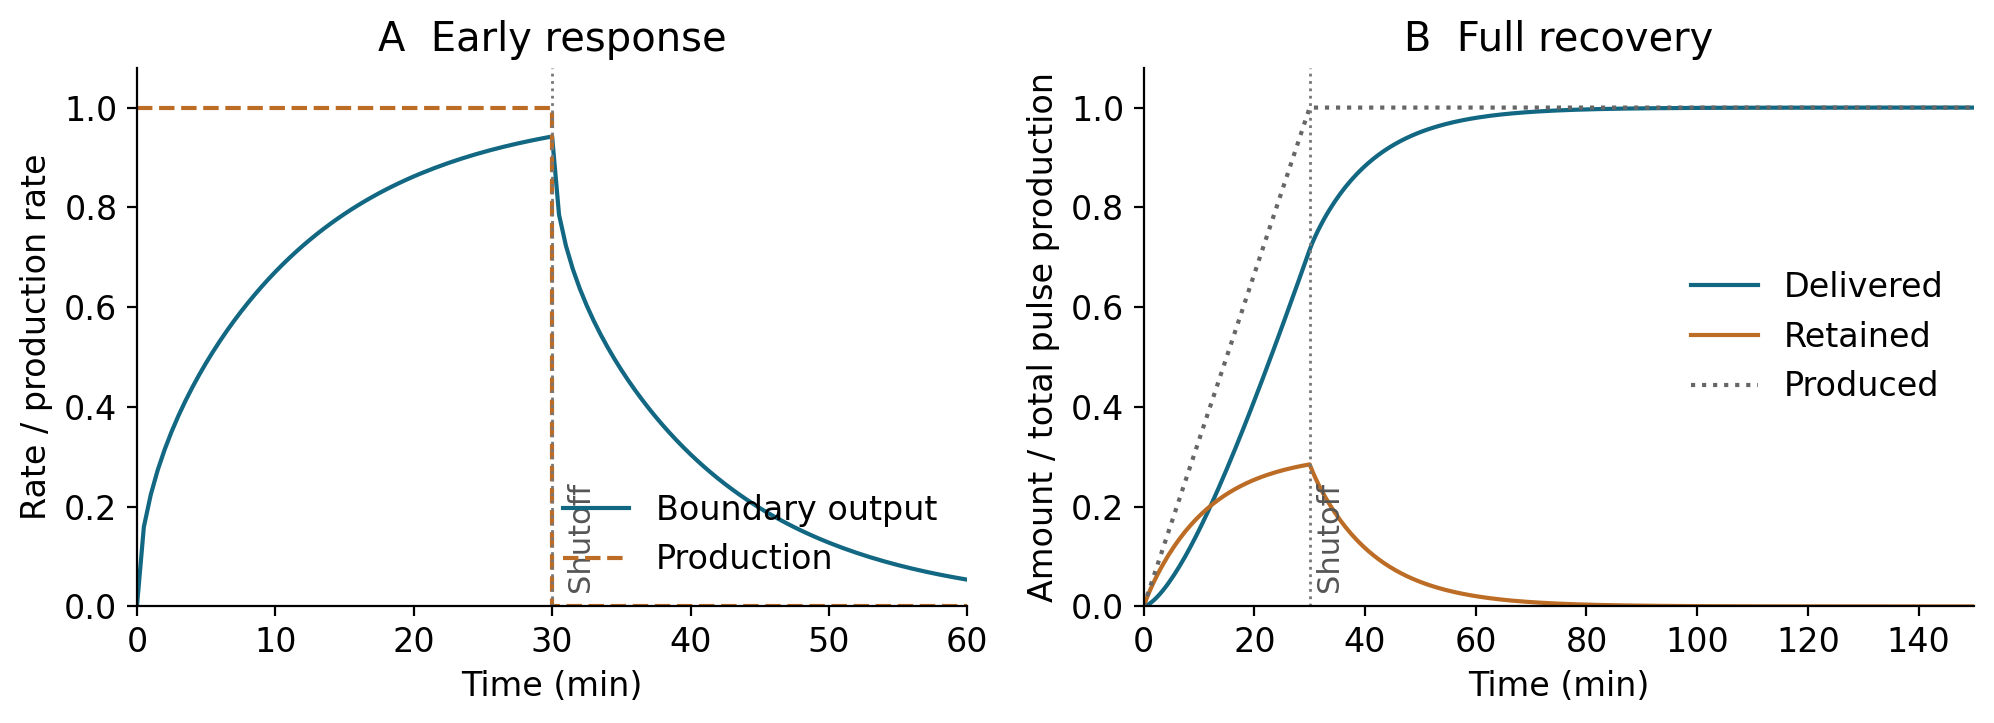
\includegraphics[width=0.9264705882352942\linewidth]{assets/production_delivery.png}\caption{Response to a fixed 30-minute production increment. A enlarges the first 60 minutes and marks shutoff; output is normalized to the fixed on-state production rate s\textsubscript{0}V. B follows cumulative production, boundary delivery and retained inventory to 150 minutes, each normalized to total pulse production. The recovery curve R\ensuremath{\tau} differs from \ensuremath{\eta}(T) for a source maintained to every deadline.}\end{figure}
The redesign family preserves N = 420,000 IEQ, \ensuremath{\rho} and b while varying h from 0.10 to 1.00 mm in 0.01 mm steps. Total length follows the fixed volume, and the minimum number of segments of at most 70 mm is used, with one shorter remainder. This prevents cost-free proliferation of absorbing end faces. In the SI length formula below, \ensuremath{\rho} = 5.38937 \ensuremath{\times} 10\textsuperscript{1}\textsuperscript{0} IEQ/m\textsuperscript{3} and radii are in metres.

\begin{equation}L_{\mathrm{tot}}(h)=\frac{N}{\rho\pi[b^2-(b-h)^2]},\qquad A_{\mathrm{lat}}=2\pi bL_{\mathrm{tot}}\end{equation}
\par\begin{table}[htbp]\centering\small Table 3. Favorable nominal scenario: minimum lateral area on the sampled grid at 30 minutes.\\[4pt]\begin{tabularx}{\linewidth}{>{\raggedright\arraybackslash}X>{\raggedright\arraybackslash}X>{\raggedright\arraybackslash}X>{\raggedright\arraybackslash}X>{\raggedright\arraybackslash}X}\toprule
Target & h (mm) & Achieved & Area (cm\textsuperscript{2}) & Grid qualification\\\midrule
50\% & 1.0 & 59.10\% & 89.92 & Thickest tested boundary\\
60\% & 0.97 & 60.40\% & 92.28 & Interior sampled minimum\\
70\% & 0.77 & 70.42\% & 112.79 & Interior sampled minimum\\
80\% & 0.6 & 80.21\% & 141.18 & Interior sampled minimum\\
90\% & 0.41 & 90.28\% & 201.07 & Interior sampled minimum\\
\bottomrule\end{tabularx}\end{table}\par
The 0.60 mm nominal choice delivers 80.21\%, only 0.21 percentage points above the benchmark. Its 141.18 cm\textsuperscript{2} lateral area is 22.28\% above nominal; its active single-row footprint is 52.85 versus 40.95 cm\textsuperscript{2} (+29.1\%), and nine versus seven pouches is +28.6\%. The 1 mm spacing and 70 mm longest segment define this footprint. It excludes the generator, connectors, manifolds, implantation clearances and tissue accommodation. These costs are not interchangeable (Figure 3).

\begin{figure}[htbp]\centering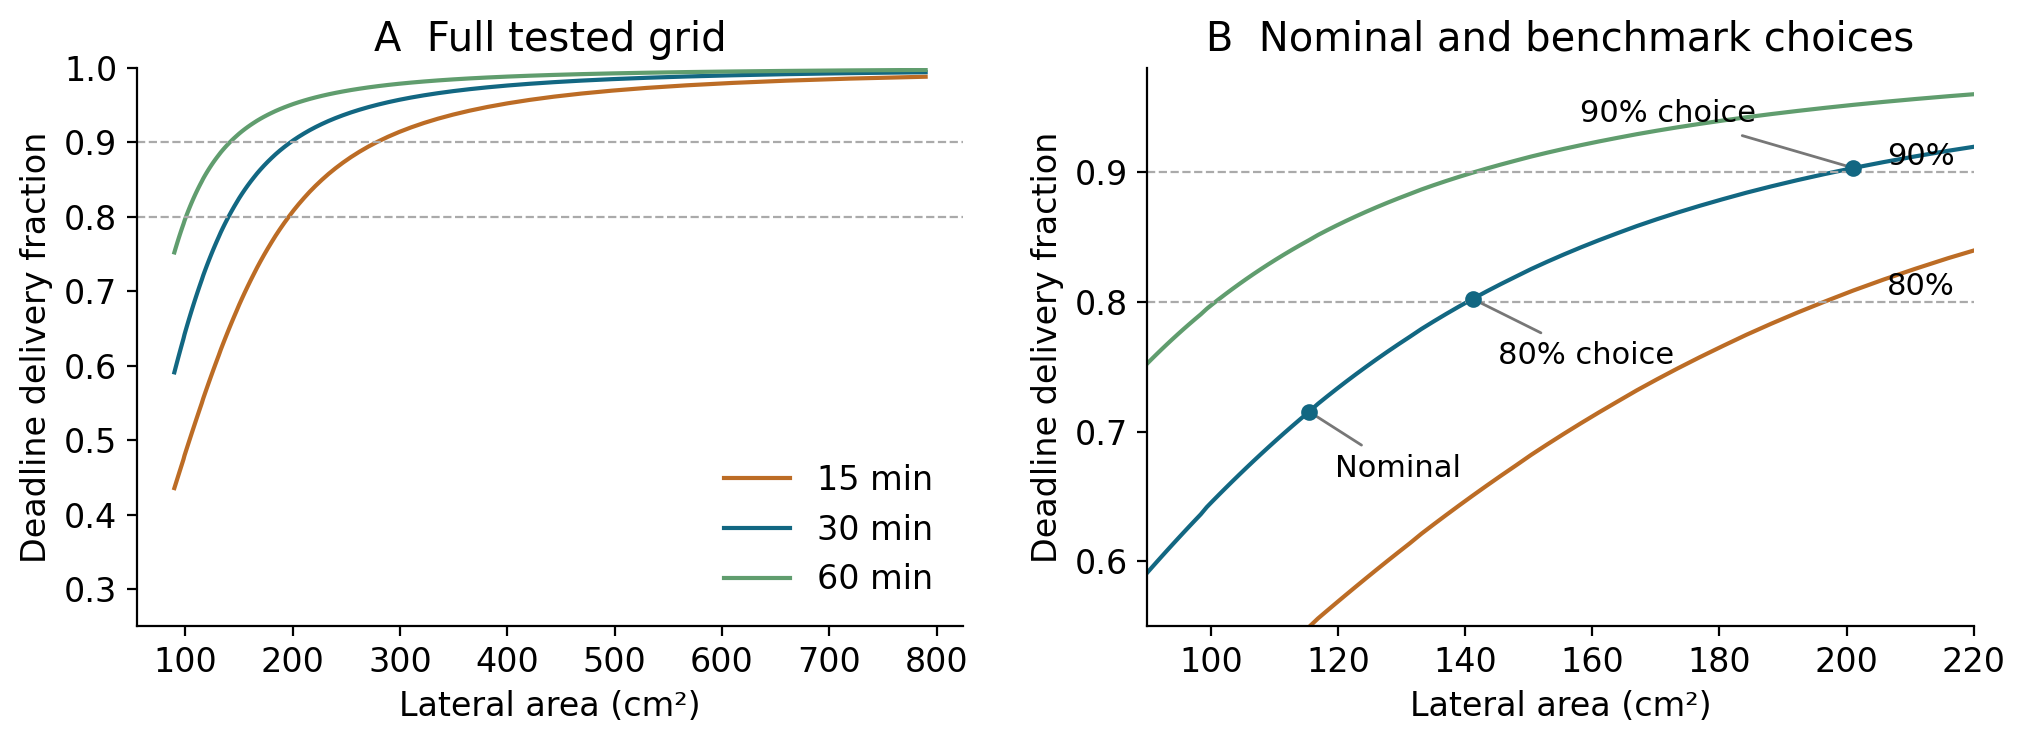
\includegraphics[width=0.9264705882352942\linewidth]{assets/dose_area_frontier.png}\caption{Favorable-scenario delivery versus lateral area at fixed dose. A shows the full tested grid; B enlarges 90--220 cm\textsuperscript{2} and marks nominal geometry and the 80\% and 90\% choices at 30 minutes. Horizontal lines are engineering benchmarks. Annular end area and system overhead are excluded from the plotted lateral area.}\end{figure}
\section*{5 Scenario-qualified design requirements}
\par\begin{table}[htbp]\centering\small Table 4. Fragility of the nominal 80\% choice. Each geometry obeys the dose-preserving rule.\\[4pt]\begin{tabularx}{\linewidth}{>{\raggedright\arraybackslash}X>{\raggedright\arraybackslash}X>{\raggedright\arraybackslash}X}\toprule
Case & 30-minute delivery & Benchmark result\\\midrule
0.60 mm; perfect sinks & 80.2062\% & Above\\
0.60 mm; reflecting ends & 79.9934\% & Below\\
0.60 mm; D reduced 5\% & 79.2497\% & Below\\
0.60 mm; D = 1.0 \ensuremath{\times} 10\textsuperscript{-}\textsuperscript{1}\textsuperscript{0} & 55.2276\% & Below\\
0.61 mm; perfect sinks & 79.6299\% & Below\\
\bottomrule\end{tabularx}\end{table}\par
The critical diffusivity for the 0.60 mm absorbing-end design to retain 80\% delivery is approximately 2.9666 \ensuremath{\times} 10\textsuperscript{-}\textsuperscript{1}\textsuperscript{0} m\textsuperscript{2}/s, only 1.1\% below the assumed nominal value. Reflecting ends yield 79.9934\%; refined continuum and finite-volume results place this below the threshold rather than a rounding ambiguity. The 0.61 mm case changes total length and segmentation to preserve dose, so it is a design-family comparison, not a measured manufacturing tolerance. The original 22.28\% area increment is therefore an idealized grid requirement, not a robust recommendation.

We evaluate all 24 combinations of D = \{1.0, 2.0, 2.85, 3.0\} \ensuremath{\times} 10\textsuperscript{-}\textsuperscript{1}\textsuperscript{0} m\textsuperscript{2}/s, P = \{10\textsuperscript{-}\textsuperscript{6}, 10\textsuperscript{-}\textsuperscript{5} m/s, perfect sink\}, and absorbing or reflecting ends, denoted S24. Subset S8 uses D = \{2.85, 3.0\} \ensuremath{\times} 10\textsuperscript{-}\textsuperscript{1}\textsuperscript{0} and P = \{10\textsuperscript{-}\textsuperscript{5} m/s, perfect sink\}, with both end conditions. F denotes the favorable single scenario. These finite sets are assumed sensitivity cases, with no measured parameter coverage or assigned probabilities. The 91 thicknesses and three deadlines produce 6,552 results.

\par\begin{table}[htbp]\centering\small Table 5. Minimum-area sampled 80\% designs at 30 minutes. Limiting combinations (D in 10\textsuperscript{-}\textsuperscript{1}\textsuperscript{0} m\textsuperscript{2}/s; P in m/s): F, D = 3, P = \ensuremath{\infty}, absorbing ends; S8, D = 2.85, P = 10\textsuperscript{-}\textsuperscript{5}, reflecting ends; S24, D = 1, P = 10\textsuperscript{-}\textsuperscript{6}, reflecting ends. Area increase is relative to the original 0.75 mm geometry.\\[4pt]\begin{tabularx}{\linewidth}{>{\raggedright\arraybackslash}X>{\raggedright\arraybackslash}X>{\raggedright\arraybackslash}X>{\raggedright\arraybackslash}X>{\raggedright\arraybackslash}X>{\raggedright\arraybackslash}X>{\raggedright\arraybackslash}X}\toprule
Set & h mm & Worst delivery & Area cm\textsuperscript{2} & Increase \% & Pouches & Footprint cm\textsuperscript{2}\\\midrule
F & 0.60 & 80.21\% & 141.18 & 22.28 & 9 & 52.85\\
S8 & 0.53 & 80.59\% & 158.22 & 37.04 & 10 & 58.80\\
S24 & 0.21 & 80.85\% & 381.79 & 230.69 & 24 & 142.10\\
\bottomrule\end{tabularx}\end{table}\par
A design qualifies when its lower numerical estimate meets the target for every set member. Every lower-area competitor must have a scenario whose upper estimate is below target; unresolved overlaps trigger refinement. The accepted map satisfies this rule and includes 70 representative, selected-worst and adjacent finite-volume checks. The original near-threshold correction is retained in the supplementary record.

The limiting combinations are shown with the selected designs in Table 5 and Figure 4. All scenario members were evaluated; the observed worst cases do not certify untested parameter values. The nominal 50\% target at 30 minutes already passes at the thickest tested layer, so that minimum is limited by the grid boundary.

\begin{figure}[htbp]\centering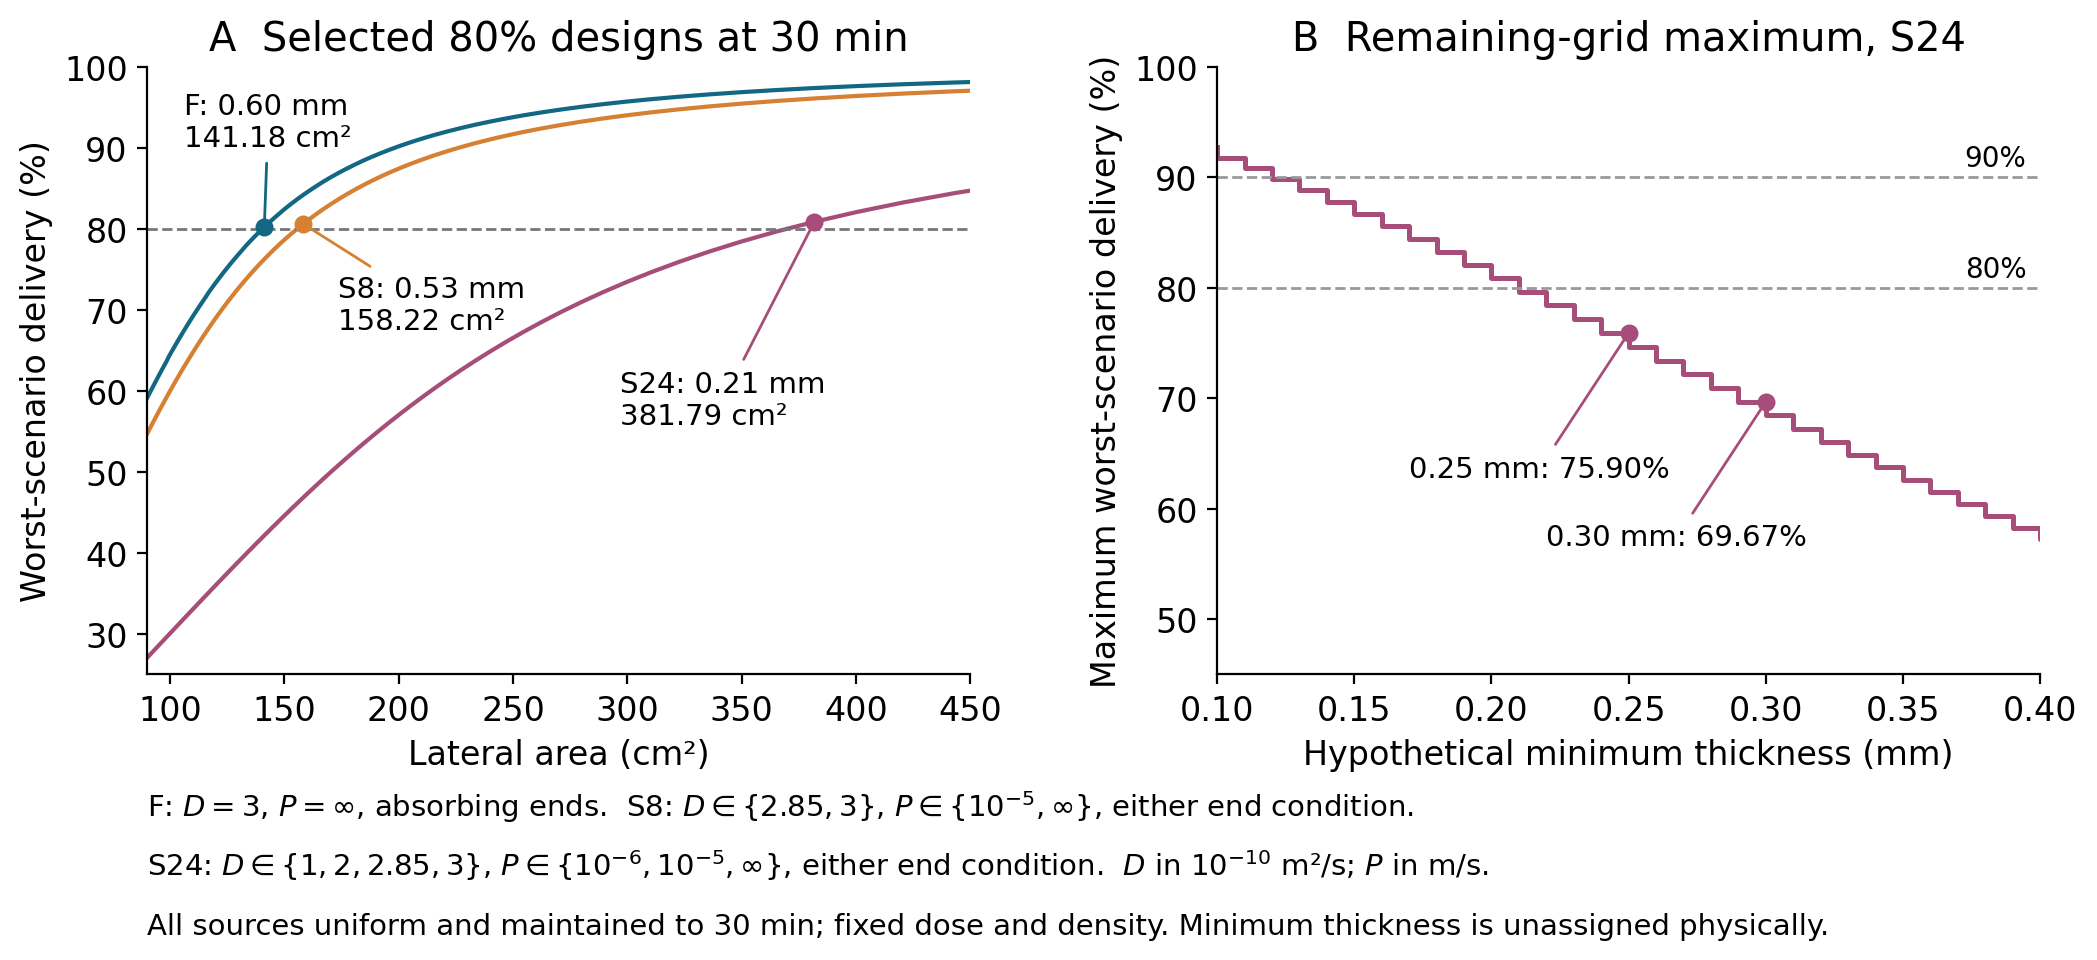
\includegraphics[width=0.9558823529411765\linewidth]{assets/design_constraints.png}\caption{A: minimum delivery across each declared set, with the selected 80\% designs labeled. B: maximum worst-scenario delivery over all remaining S24 designs satisfying the hypothetical minimum thickness. The 0.25 and 0.30 mm constraints remove every 80\% solution on this grid. Set definitions are printed in the figure; no empirical minimum thickness is assigned.}\end{figure}
\section*{6 Minimum thickness and transport mechanisms}
The S24 80\% choice has a 210 \ensuremath{\mu}m layer, only 1.4 times the IEQ reference diameter; its 90\% choice is 120 \ensuremath{\mu}m. Neither ratio decides whether an actual preparation can be loaded. Islet-size distribution, deformation, placement and clearance must determine an allowable layer thickness. We therefore leave the minimum permitted thickness as an unassigned parameter.

\begin{equation}\mathcal{H}(h_{\min})=\{h\in\mathcal{G}:h\geq h_{\min}\},\qquad E_{\max}(h_{\min})=\max_{h\in\mathcal{H}(h_{\min})}\min_{s\in\mathcal{S}}\eta_s(30\,\mathrm{min};h)\end{equation}
Here G is the original 0.10--1.00 mm grid, and S is a declared scenario set. Every remaining thickness is enumerated, retaining fixed dose, density, outer radius and segmentation. Maximum-delivery estimates use the maxima of the inherited lower and upper numerical estimates; the minimum-area selection uses the same threshold and every-competitor checks as before. The analysis spans 91 minimum-thickness values in all three sets, giving 273 maxima and 546 decisions for 80\% and 90\% targets. No additional transport simulation is required.

\par\begin{table}[htbp]\centering\small Table 6. S24 at 30 minutes after a hypothetical minimum-thickness constraint. Listed h values are the minimum-area sampled choices; not attained means all remaining designs fall below the target.\\[4pt]\begin{tabularx}{\linewidth}{>{\raggedright\arraybackslash}X>{\raggedright\arraybackslash}X>{\raggedright\arraybackslash}X>{\raggedright\arraybackslash}X}\toprule
Minimum h mm & Highest worst delivery & 80\% selection & 90\% selection\\\midrule
0.10 & 92.69\% & h = 0.21 mm & h = 0.12 mm\\
0.21 & 80.85\% & h = 0.21 mm & Not attained\\
0.25 & 75.90\% & Not attained & Not attained\\
0.30 & 69.67\% & Not attained & Not attained\\
\bottomrule\end{tabularx}\end{table}\par
With minimum thicknesses of 0.25 or 0.30 mm, the remaining-grid maximum is 75.90\% or 69.67\%. Even its upper numerical estimate is below 80\%. The target therefore cannot be recovered by adding area through further thinning within this constrained family. Changing radius, packing, segmentation or transport would define a different family. A minimum-thickness constraint is necessary input to this decision, but is not sufficient evidence of physical realizability.

\par\begin{table}[htbp]\centering\small Table 7. Separate minimum-area reoptimizations for 80\% at 30 minutes. Favorable: D = 3 \ensuremath{\times} 10\textsuperscript{-}\textsuperscript{1}\textsuperscript{0} m\textsuperscript{2}/s, perfect outer sink, absorbing ends. The individual changes are D = 1 \ensuremath{\times} 10\textsuperscript{-}\textsuperscript{1}\textsuperscript{0}, P = 10\textsuperscript{-}\textsuperscript{6} m/s, or reflecting ends. All three applies them together. No minimum thickness beyond the original grid is imposed.\\[4pt]\begin{tabularx}{\linewidth}{>{\raggedright\arraybackslash}X>{\raggedright\arraybackslash}X>{\raggedright\arraybackslash}X>{\raggedright\arraybackslash}X}\toprule
Scenario change & h mm & Area cm\textsuperscript{2} & Achieved delivery\\\midrule
Favorable & 0.60 & 141.18 & 80.21\%\\
Lower D only & 0.34 & 240.09 & 80.07\%\\
Finite P only & 0.28 & 289.12 & 80.68\%\\
Reflecting ends only & 0.59 & 143.36 & 80.58\%\\
All three changes & 0.21 & 381.79 & 80.85\%\\
\bottomrule\end{tabularx}\end{table}\par
End reflection defeats the narrowly passing 0.60 mm point, yet reoptimization restores 80\% at 0.59 mm with only 2.19 cm\textsuperscript{2} (1.55\%) more area than the favorable redesign. Lower diffusivity alone requires 98.91 cm\textsuperscript{2} more, and finite permeability alone 147.94 cm\textsuperscript{2} more. Threshold sensitivity and a large resource penalty are thus different design questions. These costs are nonadditive results of five separate optimizations; they do not rank mechanisms in an actual device.

\begin{equation}\mathrm{Fo}=\frac{DT}{h^2},\qquad \mathrm{Bi}=\frac{Ph}{D}\end{equation}
Fo compares the deadline with the internal diffusion time h\textsuperscript{2}/D. Bi compares outer permeability with internal diffusive conductance D/h; small Bi indicates relatively strong boundary resistance, while a perfect sink has infinite Bi. For fixed D and finite P, thinning raises Fo and lowers Bi: both the internal time h\textsuperscript{2}/D and boundary scale h/P improve, but boundary resistance can become relatively more important. At their selected thicknesses, the favorable and lower-D-only choices have Fo = 1.50 and 1.56; the finite-P-only choice has Fo = 6.89 and Bi = 0.93. Thus rapid internal transport does not eliminate a finite outer resistance. Annular radius ratios, segment aspect ratios and end access remain additional controls.

\section*{7 Physical uncertainty and discriminating validation}
Numerical uncertainty concerns how accurately the chosen equations are solved. Parameter uncertainty concerns D, permeability, dimensions and production distribution within that model. Structural uncertainty concerns homogeneous diffusion, discrete islets, heterogeneous secretion, tissue transport and feedback. The nominal diffusivity change from 3.0 to 1.0 \ensuremath{\times} 10\textsuperscript{-}\textsuperscript{1}\textsuperscript{0} m\textsuperscript{2}/s changes delivery from 71.53\% to 45.81\%, far more than numerical error. Thus a narrow numerical interval is not a narrow prediction interval for an actual implant.

The computed response, passive ordering argument and real-device prediction are distinct levels of inference. The first two apply within their defined model; the third requires measured correspondence of geometry, source and boundaries. Boundary flux does not itself establish physiological performance. Tissue transport, heterogeneous secretion, feedback, viable packing and a spatial oxygen field remain outside this calculation.

A discriminating experiment would first measure insulin diffusion in the gel independently of the assembled membrane. Controlled assembled-device measurements would then vary receiving conditions and thickness to separate boundary resistance from internal diffusion. Insulin should be assayed directly; a surrogate requires a predeclared equivalence test. Recovery controls must quantify retained insulin, adsorption, degradation and assay recovery so missing mass is not automatically assigned to slow diffusion.

Calibrate transport parameters on one geometry, freeze them and predict at least one held-out thickness or configuration without refitting. Predeclare cumulative delivery at 5, 15, 30 and 60 minutes, time to 50\% recovery, normalized curve error and mass-balance discrepancy as comparison metrics. Predictive acceptance tolerances should be fixed from independent assay precision and repeatability before held-out data are inspected; none is invented here. Early sampling plus retained-inventory measurement is essential. Profile likelihood or a sensitivity/Jacobian analysis should test whether D and P are separately identifiable. If they are correlated, report joint ambiguity and add independent material measurements or thickness/receiving-condition contrasts. Cell-bearing validation would subsequently require independently characterized secretion inputs and source locations. This is a proposed validation plan, not a performed experiment.

\section*{8 Oxygen and source-capacity accounting}
This accounting is separate from the insulin transport simulation. At unchanged dose and an assumed consumption of 2.1 pmol O\textsubscript{2}/min/IEQ, total oxygen demand is 0.882 \ensuremath{\mu}mol/min. If electrolysis supplies all of it with no tissue-oxygen credit, leakage or inefficiency, the stoichiometric current floor is about 5.7 mA. Voltage, conversion loss, control power and reserve are not included. Thinning does not remove this total demand; localization can increase local oxygen-delivery requirements. No spatial oxygen sufficiency follows.

Papas-derived HSA- and FBS-culture values in the BEAM supplement describe different preparations, not paired basal/stimulated states [6]. Other consumption values remain unpaired scenarios. Wang supplies dynamic oxygen-response context [7], while the Papas review surveys oxygenation strategies [8]; neither is used to invent a device-specific bound. For a symbolic external amount B required by T under the same uniform constant production, mean intrinsic secretion per IEQ must be at least B/[NT\ensuremath{\eta}(T)]. No patient demand is assigned, and hour-long external GSIS measurements are not substituted for minute-scale intrinsic secretion.

\section*{9 Reproducibility and provenance}
The package first verifies supplied files and frozen specifications by exact hashes, then regenerates the transport study and manuscripts in a separate directory. Floating-point results are compared under an explicit field-specific tolerance contract; identities, selected designs and threshold decisions must agree exactly. Reference and generated hashes are recorded separately, so last-bit numerical variation is not mistaken for altered supplied data. Reproduction tolerances do not enlarge numerical uncertainty or engineering acceptance criteria. The workflow uses pinned Python dependencies and no network or private source cache. Separate continuum and finite-volume constructions check the transport computation; they are not an external implementation or experimental validation.

The source ledger and bounded literature audit through 26 October 2026 retain exact acquisition and access limits. Trask’s accepted main text and accessible publisher sections were inspected; Papas [8] was limited to bibliographic records, abstract and publisher preview. No new references were added for the present extension, and the comparison does not establish priority.

AI assistance was used in literature retrieval, mathematical implementation, numerical checking and drafting. Separate automated review passes are disclosed as internal checks, not independent human scientific review. No new animal or human experiment was performed.

\par\noindent\begin{minipage}{\linewidth}
\section*{10 Conclusion}
In the proposed BEAM geometry, favorable passive transport delivers 71.53\% of a uniform 30-minute production increment by its deadline. Preserving dose while thinning improves delivery, but the nominal 0.60 mm design has little margin. Reoptimization distinguishes the small additional area needed after end reflection from the larger requirements in the selected lower-diffusivity and finite-permeability cases. A minimum permitted thickness can remove every target-meeting design from the sampled family: under S24, hypothetical limits of 0.25 and 0.30 mm leave no 80\% solution. The map therefore answers both how much area is needed and whether the requirement is attainable under stated constraints. Independent gel, membrane and allowable-layer measurements, followed by prediction of a held-out geometry without refitting, would identify which part of this map applies to an actual device.

\section*{References}
\par\noindent\begin{minipage}{\linewidth}\small [1] Pham TT, Tran PL, Tempelman LA, et al. A continuously oxygenated macroencapsulation system enables high-density packing and delivery of insulin-secreting cells. Nature Communications. 2025;16:7199. doi:10.1038/s41467-025-62271-2. Geometry: Supplementary Fig.24, p.21; oxygen: Supplementary Table1, p.26.\end{minipage}\par\vspace{2pt}

\par\noindent\begin{minipage}{\linewidth}\small [2] Buchwald P, Cechin SR, Weaver JD, Stabler CL. Experimental evaluation and computational modeling of the effects of encapsulation on the time-profile of glucose-stimulated insulin release of pancreatic islets. BioMedical Engineering OnLine. 2015;14:28. doi:10.1186/s12938-015-0021-9.\end{minipage}\par\vspace{2pt}

\par\noindent\begin{minipage}{\linewidth}\small [3] Ernst AU, Wang LH, Worland SC, et al. A predictive computational platform for optimizing the design of bioartificial pancreas devices. Nature Communications. 2022;13:6031. doi:10.1038/s41467-022-33760-5.\end{minipage}\par\vspace{2pt}

\par\noindent\begin{minipage}{\linewidth}\small [4] Thomson EA, Lee S, Xu H, et al. Intermittent Low-Magnitude Pressure Applied Across Macroencapsulation Devices Enables Physiological Insulin Delivery Dynamics. Diabetes. 2025;74(6):873--884. doi:10.2337/db24-0818. Supplement: doi:10.2337/figshare.28500536.\end{minipage}\par\vspace{2pt}

\par\noindent\begin{minipage}{\linewidth}\small [5] Trask L, Ward NA, Tarpey R, et al. Exploring therapy transport from implantable medical devices using experimentally informed computational methods. Biomaterials Science. 2024;12(11):2899--2913. doi:10.1039/D4BM00107A.\end{minipage}\par\vspace{2pt}

\par\noindent\begin{minipage}{\linewidth}\small [6] Papas KK, Colton CK, Nelson RA, et al. Human islet oxygen consumption rate and DNA measurements predict diabetes reversal in nude mice. American Journal of Transplantation. 2007;7(3):707--713. doi:10.1111/j.1600-6143.2006.01655.x.\end{minipage}\par\vspace{2pt}

\par\noindent\begin{minipage}{\linewidth}\small [7] Wang W, Upshaw L, Strong DM, Robertson RP, Reems J. Increased oxygen consumption rates in response to high glucose detected by a novel oxygen biosensor system in non-human primate and human islets. Journal of Endocrinology. 2005;185(3):445--455. doi:10.1677/joe.1.06092.\end{minipage}\par\vspace{2pt}

\par\noindent\begin{minipage}{\linewidth}\small [8] Papas KK, De Leon H, Suszynski TM, Johnson RC. Oxygenation strategies for encapsulated islet and beta cell transplants. Advanced Drug Delivery Reviews. 2019;139:139--156. doi:10.1016/j.addr.2019.05.002.\end{minipage}\par\vspace{2pt}

\end{minipage}
\end{document}
